%==============================================================================
% INFORME PARCIAL BME513 v8 (v8.1 - métricas CV honestas)
% Sistema local de auditoría técnica de informes mamográficos en español
% Autor: Sebastián Inostroza Hurtado
% Universidad de Valparaíso, Junio 2026
%==============================================================================

\documentclass[10pt,journal,a4paper]{IEEEtran}

\usepackage[utf8]{inputenc}
\usepackage[T1]{fontenc}
\usepackage[spanish,es-tabla,es-noindentfirst]{babel}
\usepackage{microtype}
\usepackage{graphicx}
\usepackage{booktabs}
\usepackage{array}
\usepackage{amsmath}
\usepackage{amssymb}
\usepackage{xcolor}
\usepackage{hyperref}
\usepackage{url}
\usepackage{cite}
\usepackage{listings}
\usepackage{textcomp}

\hypersetup{
    colorlinks=true,
    linkcolor=black,
    citecolor=blue,
    urlcolor=blue,
    pdftitle={Sistema local de auditoría técnica de informes mamográficos en español mediante NLP},
    pdfauthor={Sebastián Inostroza}
}

\newcommand{\birads}[1]{BI-RADS~#1}
\newcommand{\codename}[1]{\texttt{#1}}

\title{Sistema local de auditor\'ia t\'ecnica de informes mamogr\'aficos en espa\~nol mediante NLP: coherencia entre la categor\'ia BI-RADS y la recomendaci\'on cl\'inica}

\author{
    Sebasti\'an Inostroza Hurtado
    \thanks{Doctorado en Ciencias e Ingenier\'ia para la Salud, Universidad de Valpara\'iso, Valpara\'iso, Chile. (e-mail: sebastian.inostroza@postgrado.uv.cl). Trabajo desarrollado para el curso BME513 --- Inteligencia Artificial en Salud.}
}

\markboth{Curso BME513, Universidad de Valpara\'iso}{Inostroza: Auditor\'ia t\'ecnica de informes mamogr\'aficos}

\begin{document}

\maketitle

\begin{abstract}
El c\'ancer de mama es la principal causa de mortalidad oncol\'ogica femenina en Am\'erica Latina. La informaci\'on cr\'itica de los informes mamogr\'aficos (la categor\'ia BI-RADS y la recomendaci\'on cl\'inica) queda habitualmente atrapada como texto libre, lo que dificulta su explotaci\'on por sistemas administrativos y la detecci\'on autom\'atica de inconsistencias entre el diagn\'ostico y la conducta sugerida. Este trabajo presenta un sistema de procesamiento de lenguaje natural ejecutable localmente que audita t\'ecnicamente la coherencia interna de los informes mamogr\'aficos en espa\~nol, contrastando la categor\'ia BI-RADS declarada por el radi\'ologo con la recomendaci\'on cl\'inica emitida bajo el est\'andar BI-RADS/ACR. El objetivo es una herramienta aplicable a la sem\'antica cl\'inico-radiol\'ogica latinoamericana, con Chile como contexto de despliegue previsto, apoy\'andose en la uniformidad regional que induce la adopci\'on del est\'andar BI-RADS/ACR. El pipeline integra cuatro m\'odulos: un extractor de categor\'ia BI-RADS por reglas con tolerancia a variaciones tipogr\'aficas; un extractor de recomendaciones con tres capas de procesamiento (normalizaci\'on, reglas cl\'inicas y similitud sem\'antica TF-IDF); un motor de cotejo contra una tabla que formaliza el est\'andar BI-RADS/ACR; y un extractor NER basado en DistilBETO que localiza la recomendaci\'on en redacciones no anticipadas por las reglas. Evaluado sobre 4\,357 informes en espa\~nol de un corpus p\'ublico paraguayo, el sistema alcanz\'o Macro F1 de 0,9995 en la extracci\'on de BI-RADS por reglas y F1 de span de 0,9991 en la localizaci\'on neuronal de la recomendaci\'on. Un verificador Transformer entrenado para contrastar la extracci\'on reglada (Macro F1 = 0,8877 $\pm$ 0,0501 bajo validaci\'on cruzada de 5 particiones) se retir\'o del pipeline tras medir por cuatro v\'ias que no aporta sobre las reglas, resultado que se reporta por su valor metodol\'ogico. El sistema gener\'o alertas cl\'inicas en el 1,15\,\% de los informes, un nivel bajo de fatiga de alertas. La ejecuci\'on local facilita el cumplimiento de normativas de protecci\'on de datos como la Ley N.\textsuperscript{o}~19.628 en Chile. Como limitaci\'on, el corpus es de origen paraguayo y no chileno, por lo que la validaci\'on sobre informes locales queda como trabajo futuro. El resultado es una herramienta interpretable y auditable de control de calidad para programas de tamizaje mamogr\'afico.
\end{abstract}

\begin{IEEEkeywords}
NLP cl\'inico, BI-RADS, informes mamogr\'aficos, auditor\'ia t\'ecnica, DistilBETO, espa\~nol cl\'inico, salud digital.
\end{IEEEkeywords}

\section{Introducci\'on}\label{sec:intro}
\IEEEPARstart{E}{l} c\'ancer de mama es la primera causa de mortalidad por tumores malignos en mujeres en Am\'erica Latina, y en Chile en particular exhibe tasas con un crecimiento sostenido en la \'ultima d\'ecada \cite{deis2024}. El tamizaje mamogr\'afico constituye la principal estrategia poblacional de detecci\'on temprana, y la calidad del informe radiol\'ogico --particularmente la categor\'ia BI-RADS asignada y la recomendaci\'on cl\'inica emitida-- determina directamente la conducta de seguimiento. Garantizar la coherencia interna entre estos dos elementos es, por tanto, una preocupaci\'on cl\'inica de primer orden en toda la regi\'on.

En la pr\'actica asistencial, los informes mamogr\'aficos se generan como texto libre estructurado en bloques (hallazgos, conclusi\'on, recomendaciones), donde la categor\'ia BI-RADS y la recomendaci\'on cl\'inica quedan atrapadas en lenguaje natural. Esto dificulta su explotaci\'on por sistemas administrativos del centro asistencial y, m\'as relevante, imposibilita la auditor\'ia autom\'atica de coherencia entre lo que el radi\'ologo concluy\'o y lo que recomend\'o. Un BI-RADS 4 (sospechoso) acompa\~nado de una recomendaci\'on de \emph{control anual} ilustra el tipo de inconsistencia que un sistema de validaci\'on t\'ecnica podr\'ia detectar, y que actualmente solo se identifica mediante revisi\'on manual.

El procesamiento de lenguaje natural (NLP) aplicado a informes radiol\'ogicos ha sido investigado principalmente en ingl\'es. Sippo et al. \cite{sippo2013} demostraron la viabilidad de la extracci\'on regex de categor\'ias BI-RADS con recall del 100\% y precisi\'on del 96,6\%; Kuling et al. \cite{kuling2022} desarrollaron BI-RADS BERT con segmentaci\'on de secciones logrando 98\% de acierto en clasificaci\'on de secciones. En espa\~nol, L\'opez-\'Ubeda et al. \cite{lopez2024} reportaron Macro F1 de 0,74 utilizando BETO sobre corpus espa\~nol peninsular para clasificaci\'on de BI-RADS. Sin embargo, la mayor\'ia de los trabajos publicados abordan la \emph{predicci\'on} de la categor\'ia BI-RADS desde el texto, no la \emph{auditor\'ia} de su coherencia con la conducta cl\'inica recomendada.

Dos hechos justifican la relevancia de esta auditor\'ia. Primero, en Chile el sistema BI-RADS no es opcional en la pr\'actica: la Gu\'ia de Pr\'actica Cl\'inica AUGE de C\'ancer de Mama del Ministerio de Salud clasifica los hallazgos mamogr\'aficos seg\'un las categor\'ias BI-RADS y asocia cada una a una conducta --por ejemplo, los BI-RADS 4 y 5 deben derivarse como casos GES-- de modo que el registro estad\'istico nacional y el flujo asistencial dependen de esta categorizaci\'on \cite{minsal2015gpc}. La coherencia entre categor\'ia y conducta es, por tanto, un requisito operativo, no solo una buena pr\'actica. Segundo, aunque el BI-RADS estandariza el lenguaje, no elimina la variabilidad entre observadores: distintos radi\'ologos ante la misma imagen alcanzan solo una concordancia moderada en la evaluaci\'on final, y esta var\'ia seg\'un el tipo de hallazgo \cite{berg2000birads, lazarus2006birads}. Una herramienta que verifique de forma objetiva y reproducible la coherencia interna del informe aporta, en ese contexto, una capa de control de calidad que la interpretaci\'on humana por s\'i sola no garantiza. El alcance del sistema es acotado. No juzga si la categor\'ia BI-RADS fue bien asignada --esa es la parte sujeta a variabilidad humana--, sino que, dada la categor\'ia declarada, verifica que la recomendaci\'on sea consistente con ella, aislando as\'i la componente auditable y objetiva del problema.

El problema espec\'ifico que motiva este trabajo es distinto: dado un informe ya emitido por un radi\'ologo, verificar autom\'aticamente si la categor\'ia BI-RADS declarada y la recomendaci\'on cl\'inica son coherentes seg\'un el est\'andar BI-RADS/ACR \cite{acr2013}. Esto se enmarca dentro de un programa m\'as amplio de auditor\'ia de informes mamogr\'aficos; en una l\'inea complementaria, el autor desarrolla en paralelo, dentro de otro curso, trabajo sobre auditor\'ia de coherencia diagn\'ostica.

Este art\'iculo presenta el dise\~no, la implementaci\'on y la validaci\'on de un sistema local de auditor\'ia t\'ecnica de informes mamogr\'aficos en espa\~nol. La propuesta integra cuatro m\'odulos: un extractor de categor\'ia BI-RADS basado en reglas y robusto a variaciones tipogr\'aficas; un extractor de recomendaciones que combina normalizaci\'on, reglas cl\'inicas y similitud sem\'antica; un motor de cotejo contra una tabla que formaliza el est\'andar BI-RADS/ACR; y un extractor NER basado en DistilBETO que localiza la recomendaci\'on en redacciones no anticipadas por las reglas. Todo el procesamiento ocurre localmente, sin enviar datos sensibles a servicios externos, lo que facilita el cumplimiento de normativas de protecci\'on de datos como la Ley N.\textsuperscript{o}~19.628 en Chile, contexto de despliegue previsto \cite{ley19628}. Se opt\'o por un motor reglado como columna vertebral en lugar de un enfoque generativo porque la tarea es esencialmente determinista: localizar una categor\'ia declarada de forma expl\'icita y cotejarla contra una norma fija. Adem\'as, el dominio cl\'inico exige transparencia, reproducibilidad y auditabilidad, propiedades que un modelo generativo comprometer\'ia al introducir opacidad, comportamiento no determinista y riesgo de alucinaci\'on.

Las contribuciones principales son cuatro. Primera, la formalizaci\'on computacional del est\'andar BI-RADS/ACR en una tabla auditable de conductas esperadas, equivalencias aceptables y niveles de severidad, aplicable a informes en espa\~nol gracias a la uniformidad regional del lenguaje cl\'inico-radiol\'ogico y pendiente de validaci\'on cl\'inica formal. Segunda, una arquitectura donde las reglas resuelven la extracci\'on de la categor\'ia y el aprendizaje autom\'atico queda acotado al m\'odulo donde la variaci\'on es sem\'antica, con una tasa de alerta del 1,15\,\% sobre el corpus que mantiene baja la fatiga de alertas. Tercera, un resultado negativo medido: se entren\'o y evalu\'o un verificador Transformer para la extracci\'on de BI-RADS y cuatro pruebas independientes muestran que no aporta sobre la v\'ia reglada, por lo que se retir\'o del pipeline y se documenta con la causa identificada. Cuarta, la evaluaci\'on emp\'irica sobre un corpus p\'ublico de 4\,357 informes en espa\~nol \cite{vazquez2025}, con validaci\'on cruzada estratificada para reportar m\'etricas libres del sesgo de selecci\'on de checkpoint, complementada por una bater\'ia de casos sint\'eticos que verifica la cobertura sobre variantes de formato ausentes del corpus y permite reproducir esa verificaci\'on sin acceso a datos cl\'inicos.

El resto del art\'iculo se estructura como sigue. La Secci\'on II describe el dataset y la metodolog\'ia. La Secci\'on III presenta los resultados experimentales y su discusi\'on. La Secci\'on IV resume las conclusiones y delinea el trabajo futuro.

\section{Materiales y M\'etodos}

\subsection{Materiales}

\subsubsection{Dataset}
Se utiliz\'o el corpus p\'ublico \emph{Mammography reporting dataset with BI-RADS system} \cite{vazquez2025}, disponible en Zenodo (DOI 10.5281/zenodo.14827680). El corpus contiene 4\,357 informes mamogr\'aficos reales en espa\~nol, anonimizados, provenientes de un centro asistencial paraguayo y emitidos entre 2019 y 2024, con etiqueta BI-RADS 0--6 y campo \texttt{Recommendations} con la conducta cl\'inica sugerida.

La elecci\'on de este corpus responde a su disponibilidad p\'ublica y volumen sustancial, en ausencia de datasets chilenos abiertos comparables al momento de este trabajo. El objetivo del sistema es operar sobre la sem\'antica cl\'inico-radiol\'ogica latinoamericana en espa\~nol --incluido Chile como contexto de despliegue previsto--, apoy\'andose en la alta uniformidad regional que induce la adopci\'on internacional del est\'andar BI-RADS/ACR: los patrones ling\"u\'isticos y las categorizaciones identificadas son razonablemente extrapolables entre contextos hispanohablantes de la regi\'on. No obstante, se reconoce expl\'icitamente como \textbf{limitaci\'on} que el corpus es de origen \emph{paraguayo} y no chileno; por tanto, aunque el est\'andar compartido favorece la transferibilidad, las particularidades de redacci\'on de cada centro o pa\'is podr\'ian diferir. El refinamiento y la validaci\'on del sistema sobre informes mamogr\'aficos chilenos, con radi\'ologos locales, quedan identificados como trabajo futuro.

La distribuci\'on de etiquetas est\'a marcadamente desbalanceada: BI-RADS 2 concentra 2\,635 informes (60,5\%), seguido de BI-RADS 0 (966, 22,2\%) y BI-RADS 1 (596, 13,7\%). Las clases cl\'inicamente cr\'iticas son minoritarias: BI-RADS 4 (52 informes, 1,2\%), BI-RADS 3 (87, 2,0\%), BI-RADS 5 (16, 0,4\%) y BI-RADS 6 (5, 0,1\%). Este desbalance motiv\'o el uso de Macro F1 como m\'etrica principal y la aplicaci\'on de aumentaci\'on textual durante el entrenamiento del modelo Transformer.

\subsubsection{Modelo Transformer y protocolo de evaluaci\'on}
Se utiliz\'o DistilBETO (\texttt{dccuchile/distilbert-base-spanish-uncased}) \cite{canete2020}, una versi\'on destilada de BETO siguiendo el esquema DistilBERT \cite{sanh2019}, como modelo base, fine-tuneado sobre el corpus de entrenamiento con tres \'epocas, batch size 8, learning rate $2\times10^{-5}$, y aumentaci\'on textual sobre clases minoritarias mediante diccionarios de sin\'onimos cl\'inicos. La elecci\'on de DistilBETO sobre alternativas como BETO completo o XLM-RoBERTa se justifica por su menor huella computacional (\textasciitilde 250 MB), su entrenamiento espec\'ifico en espa\~nol y la disponibilidad de aceleraci\'on local mediante Metal Performance Shaders (MPS) de Apple Silicon.

Bajo un split estratificado 80/20 \'unico, el mejor modelo alcanz\'o Macro F1 = 0,9386 sobre el conjunto de prueba (872 informes). Este esquema, sin embargo, usa el mismo conjunto de prueba para seleccionar el punto de control y para la evaluaci\'on final, por lo que la m\'etrica resultante puede quedar algo optimizada. Para obtener una evaluaci\'on libre de ese sesgo se realiz\'o adem\'as una validaci\'on cruzada estratificada de 5 particiones (con semilla fija), aplicando la aumentaci\'on textual dentro de cada partici\'on y no de forma global, de modo que las variantes l\'exicas de un mismo informe no se repartieran entre entrenamiento y prueba. La m\'etrica honesta resultante es \textbf{Macro F1 = 0,8877 $\pm$ 0,0501}, que es la del clasificador finalmente descartado (Secci\'on~\ref{sec:verif}). La diferencia respecto del split \'unico ($-0,0509$) es la esperable al eliminar el sesgo de selecci\'on.

\subsubsection{Tabla normativa BI-RADS/ACR}
Se construy\'o una formalizaci\'on computacional de las recomendaciones de manejo del Atlas BI-RADS de la American College of Radiology \cite{acr2013}. La tabla mapea cada categor\'ia BI-RADS (0--6) a una recomendaci\'on esperada, un conjunto de equivalentes cl\'inicamente aceptables, subcategor\'ias de notificaci\'on suave y un nivel de severidad de alerta, a partir del est\'andar ACR y de la literatura cl\'inica. Por ejemplo, BI-RADS 4 acepta como recomendaci\'on esperada \emph{biopsia hist\'ologica}, con \emph{derivaci\'on oncol\'ogica} como equivalente cl\'inicamente aceptable; BI-RADS 5, en cambio, se trata de forma estricta sin equivalentes dada su criticidad cl\'inica. El esquema de equivalencias y de severidades constituye una propuesta del autor derivada del est\'andar, calibrada emp\'iricamente contra el corpus (tasa de alertas del 1,15\,\%) y \textbf{pendiente de validaci\'on cl\'inica formal por radi\'ologos}, la cual se identifica como trabajo futuro.

Dada la uniformidad regional del lenguaje cl\'inico-radiol\'ogico hispano y la adopci\'on internacional del est\'andar BI-RADS/ACR, esta formalizaci\'on resulta aplicable al corpus utilizado, con el horizonte de refinamiento futuro mediante validaci\'on espec\'ifica con radi\'ologos chilenos sobre corpus locales.

\subsection{M\'etodos}
El sistema se organiza como un pipeline secuencial de cuatro m\'odulos independientes y auditables, dise\~nados bajo una filosof\'ia de \emph{Human-on-the-Loop}: el sistema detecta inconsistencias pero no decide la conducta cl\'inica. La Fig.~\ref{fig:pipeline} presenta el flujo general de datos, y la Fig.~\ref{fig:modulos} detalla la funci\'on y las herramientas de cada m\'odulo. A continuaci\'on se describe cada uno.

\begin{figure*}[!t]
\centering
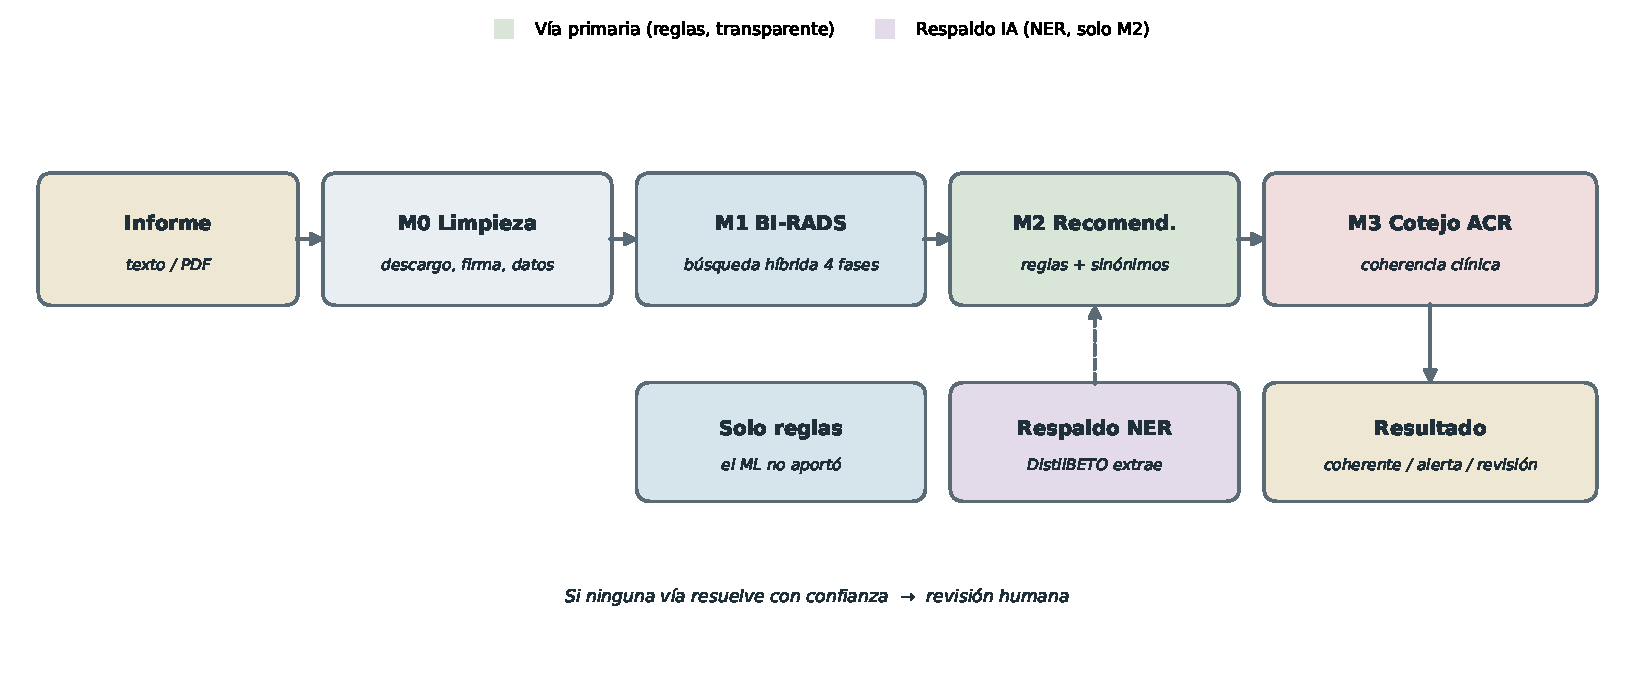
\includegraphics[width=0.92\textwidth]{figuras/fig_arq_pipeline.pdf}
\caption{Flujo general del pipeline de auditor\'ia. El informe atraviesa los m\'odulos en secuencia; el M\'odulo~4 act\'ua como verificaci\'on cruzada del BI-RADS, y las recomendaciones no clasificables con confianza se derivan a revisi\'on humana.}
\label{fig:pipeline}
\end{figure*}

\begin{figure*}[!t]
\centering
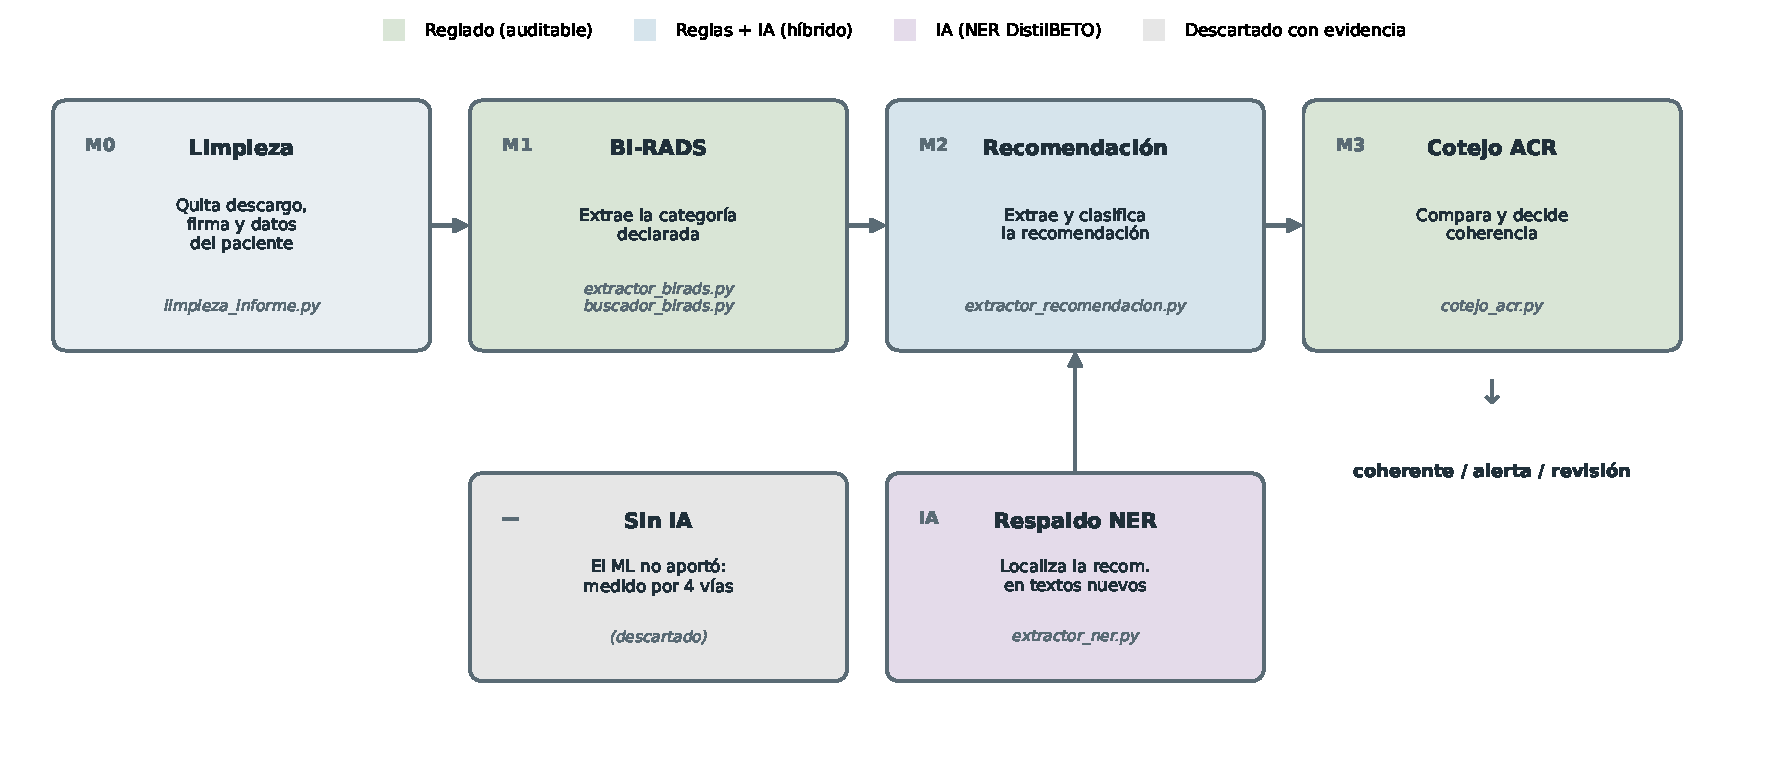
\includegraphics[width=0.82\textwidth]{figuras/fig_arq_modulos.pdf}
\caption{Arquitectura modular. El flujo (M0 a M3) es reglado y auditable. Un modelo DistilBETO respalda al M\'odulo~2 localizando la recomendaci\'on en redacciones no anticipadas. El M\'odulo~1 opera solo con reglas: el verificador Transformer que se prob\'o para \'el se retir\'o tras medir que no aporta (Secci\'on~\ref{sec:verif}).}
\label{fig:modulos}
\end{figure*}

\subsubsection{M\'odulo 0: Preprocesamiento y limpieza (\codename{limpieza\_informe.py})}
Antes de cualquier extracci\'on, el informe pasa por una capa de limpieza que elimina las l\'ineas sin contenido cl\'inico: el descargo legal frecuente en informes chilenos (``el presente resultado debe correlacionarse con el cuadro cl\'inico''), la firma y validaci\'on del m\'edico, la paginaci\'on y los datos administrativos del paciente. La limpieza opera por l\'ineas y no por rangos, porque la extracci\'on de texto desde un PDF puede alterar el orden y ubicar el pie de p\'agina al inicio. El dise\~no es conservador: cada patr\'on identifica una l\'inea inequ\'ivocamente administrativa, y una salvaguarda impide eliminar contenido cuando las coincidencias superan el 60\,\% de las l\'ineas.

Esa salvaguarda protege el contenido cl\'inico, pero entra en conflicto con la protecci\'on de datos personales. Cuando el nombre del radi\'ologo o un identificador quedan en la misma l\'inea que la conclusi\'on, algo habitual al extraer de un PDF, eliminar la l\'inea completa se llevar\'ia tambi\'en la categor\'ia BI-RADS. La salvaguarda lo impide, y el identificador sobrevive. Las dos protecciones se anulan entre s\'i.

El m\'odulo incorpora por eso una segunda capa que redacta dentro de la l\'inea en lugar de eliminarla, sustituyendo el fragmento identificatorio por una etiqueta gen\'erica y conservando intacto el texto cl\'inico. Cubre el nombre del profesional con sus tratamientos habituales, el identificador nacional en sus formatos usuales y los campos administrativos en l\'inea. La redacci\'on se aplica tambi\'en cuando la salvaguarda revierte la eliminaci\'on, que era el caso desprotegido. Sobre el corpus completo la capa no produce falsos positivos, y el texto cl\'inico permanece sin alterar. Con ambas capas, el sistema reduce el manejo de datos personales en concordancia con la Ley N.\textsuperscript{o} 19.628.

\subsubsection{M\'odulo 1: Extractor de BI-RADS (\codename{extractor\_birads.py}, \codename{buscador\_birads.py})}
La tarea de este m\'odulo es encontrar, dentro del texto libre, la categor\'ia BI-RADS que el radi\'ologo asign\'o. Es el n\'ucleo del sistema: define la vara contra la que el M\'odulo~3 mide la recomendaci\'on. Opera solo con reglas y alcanza Macro F1 = 0,9995.

La primera versi\'on (\codename{extractor\_birads.py}) localiza el bloque de conclusi\'on por su encabezado y busca la categor\'ia dentro de \'el, aplicando una jerarqu\'ia que va del formato can\'onico (\emph{BI-RADS X}) a variantes tipogr\'aficas frecuentes (\emph{BR-X}, \emph{Categor\'ia X}, \emph{BI-RADS$^\circledR$ X}, n\'umeros romanos o la categor\'ia escrita en palabras). Sobre el corpus paraguayo esa estrategia cubre el 100\,\% de los informes, porque todos traen encabezado expl\'icito (\emph{Conclusi\'on} en el 67,7\,\% y \emph{Valoraci\'on} en el 32,3\,\%). Los primeros informes chilenos revelaron el l\'imite: algunos usan \emph{Impresi\'on Diagn\'ostica}, otros carecen de encabezado, y varios mencionan la categor\'ia m\'as de una vez, con una referencia hist\'orica antes de la definitiva. La dependencia del encabezado era invisible dentro del corpus de entrenamiento.

La versi\'on en uso (\codename{buscador\_birads.py}) elimina esa dependencia con una b\'usqueda en cuatro fases. La primera recorre el informe completo y recoge todas las menciones. La segunda descarta por contexto las hist\'oricas, las comparativas, las educacionales y las negadas, atendiendo a las palabras que las preceden. La tercera pondera las restantes por su posici\'on relativa: la categor\'ia definitiva aparece al final del informe, y sobre el corpus la \'ultima menci\'on se ubica en el percentil 0,85 del texto en el 100\,\% de los casos. La cuarta reserva un arbitraje para los empates, que sobre 4\,357 informes no llegan a producirse porque el 99,9\,\% declara una sola menci\'on.

Cada extracci\'on queda etiquetada con un nivel de confianza (alta en el 98,58\,\% de los informes, baja en el 1,38\,\%) seg\'un el patr\'on que la produjo, de modo que los m\'odulos siguientes puedan ponderarla. Si el informe presenta hallazgos radiol\'ogicos o recomendaciones pero no declara ninguna categor\'ia, el m\'odulo genera una alerta de omisi\'on: un estudio con hallazgos deber\'ia concluir siempre en un BI-RADS, y su ausencia apunta a un problema de documentaci\'on que corresponde resolver a una persona y no a una imputaci\'on autom\'atica.

\subsubsection{M\'odulo 2: Extractor y clasificador de recomendaciones (\codename{extractor\_recomendacion.py})}
Este m\'odulo cumple dos funciones encadenadas: primero localiza el texto de la recomendaci\'on dentro del informe y luego lo clasifica en una de ocho categor\'ias cl\'inicas, ordenadas de la m\'as urgente a la menos urgente (biopsia hist\'ologica, derivaci\'on oncol\'ogica, estudio complementario de imagen, correlaci\'on ecogr\'afica, comparaci\'on con estudios previos, control a corto plazo, control anual y criterio m\'edico). La localizaci\'on no depende de que exista un encabezado fijo de ``Recomendaciones'': si el informe no lo tiene, un mecanismo de respaldo recorre el texto en busca de frases gatillo de conducta (verbos como \emph{se sugiere}, \emph{amerita}, \emph{conviene} o \emph{derivar}), lo que permite operar sobre informes de estructura at\'ipica, un aspecto cr\'itico para su uso sobre datos externos.

La clasificaci\'on se apoya en un vocabulario cl\'inico validado y en reglas que capturan la intenci\'on del texto. Incorpora varias defensas frente a la variabilidad de la redacci\'on real: tolerancia a errores ortogr\'aficos mediante distancia de edici\'on de Damerau-Levenshtein (con umbral $\leq 1$, restringida a los verbos gatillo y nunca a cifras, para no alterar plazos ni categor\'ias), reconocimiento de directivas expresadas como sustantivo de acci\'on sin verbo introductorio (por ejemplo, \emph{``control en 3 meses''}), y detecci\'on de negaci\'on al estilo NegEx para descartar menciones negadas. A esto se suma una capa de sin\'onimos cl\'inicos que normaliza t\'erminos equivalentes a una forma can\'onica antes de aplicar las reglas: variantes de una misma t\'ecnica (\emph{ultrasonido}, \emph{US} y \emph{ecotomograf\'ia} para ecograf\'ia; \emph{RMN} y \emph{MRI} para resonancia), abreviaturas de biopsia (\emph{BACAF}, \emph{PAAF}, \emph{core biopsy}) y equivalencias de conducta (\emph{seguimiento} por control, \emph{en un a\~no} por anual). Los sin\'onimos se anclaron con contexto para evitar reescrituras err\'oneas y se excluyeron deliberadamente t\'erminos cl\'inicamente ambiguos. Cuando ninguna regla clasifica el texto con confianza, la recomendaci\'on se marca como ambigua y se deriva a revisi\'on, en lugar de forzar una categor\'ia que podr\'ia ser err\'onea.

\paragraph{Extractor NER de respaldo (\codename{extractor\_ner.py}).}
La localizaci\'on por reglas es transparente y r\'apida, pero exige anticipar cada forma de redacci\'on. Para las redacciones no vistas se incorpor\'o un extractor neuronal que act\'ua como v\'ia de respaldo: un modelo DistilBETO afinado para reconocimiento de entidades (NER) que localiza el fragmento de recomendaci\'on dentro del informe. A diferencia de las reglas, el modelo aprende el contexto de lo que es una recomendaci\'on y generaliza a formas que no estaban en el vocabulario. Su entrenamiento no requiri\'o etiquetado manual: como la recomendaci\'on aparece textualmente dentro del informe, las etiquetas por token se derivaron autom\'aticamente alineando la columna de recomendaci\'on del corpus. La arquitectura resultante es h\'ibrida y sigue la misma l\'ogica que el m\'odulo de BI-RADS: las reglas son la v\'ia primaria y, cuando no localizan la recomendaci\'on, el NER la extrae; si ninguno lo logra con confianza, el caso se deriva a revisi\'on humana. Una salvaguarda de posprocesamiento toma \'unicamente el primer fragmento contiguo etiquetado, de modo que etiquetas dispersas ante elementos no vistos (firmas, encabezados) no contaminen la extracci\'on.

\subsubsection{M\'odulo 3: Motor de cotejo BI-RADS/ACR (\codename{cotejo\_acr.py})}
Este m\'odulo es el n\'ucleo de la auditor\'ia. Recibe la categor\'ia BI-RADS extra\'ida y la recomendaci\'on ya clasificada, y decide si ambas son coherentes seg\'un el est\'andar ACR. El m\'odulo no eval\'ua si el BI-RADS est\'a bien asignado ni juzga los hallazgos. Toma el BI-RADS tal como viene y verifica \'unicamente que la recomendaci\'on sea consistente con \'el. El BI-RADS funciona, entonces, como la vara contra la que se mide la recomendaci\'on, no como algo a medir.

Para ello, cada categor\'ia BI-RADS tiene en la tabla una conducta esperada seg\'un la norma, una lista de equivalentes aceptables, otra de equivalentes que ameritan una notificaci\'on suave, y un conjunto de conductas que se marcan para revisi\'on. El motor recorre estas opciones en orden de prioridad cl\'inica, como ilustra la Fig.~\ref{fig:cotejo}, y se detiene en la primera que aplica:
\begin{enumerate}
    \item Si la recomendaci\'on coincide con la esperada, es coherente y no se emite alerta.
    \item Si no coincide pero figura entre los equivalentes aceptables (por ejemplo, la derivaci\'on oncol\'ogica en un BI-RADS 5, dado que el especialista ordenar\'a la biopsia), tambi\'en es coherente.
    \item Si figura entre los equivalentes que ameritan menci\'on, es una incoherencia leve: se emite una alerta de baja prioridad.
    \item Si es una conducta marcada para revisi\'on (por ejemplo, una acci\'on invasiva sobre un hallazgo benigno), se genera una alerta de revisi\'on.
    \item Si la recomendaci\'on es m\'as cauta que la esperada y no cae en el caso anterior, se acepta con precauci\'on, sin alerta, porque exceder la cautela rara vez es riesgoso.
    \item Si nada de lo anterior aplica, la recomendaci\'on se queda corta frente a lo que pide la norma, y se genera una alerta cuya gravedad se grad\'ua seg\'un el impacto en salud.
\end{enumerate}

El principio que ordena todo es cl\'inico: quedarse corto, es decir, recomendar una conducta menos urgente de la necesaria, es el escenario peligroso, porque puede retrasar el diagn\'ostico de un c\'ancer. Pasarse de cauto casi nunca lo es. Por eso el sistema es tolerante hacia la precauci\'on de m\'as y estricto hacia la de menos.

Toda la l\'ogica cl\'inica reside en la tabla y no en el c\'odigo, de modo que un especialista puede leerla y corregirla sin tocar el programa. Cada salida, adem\'as, registra la regla exacta que se aplic\'o, lo que hace auditable no solo la alerta sino su justificaci\'on.

\begin{figure*}[!t]
\centering
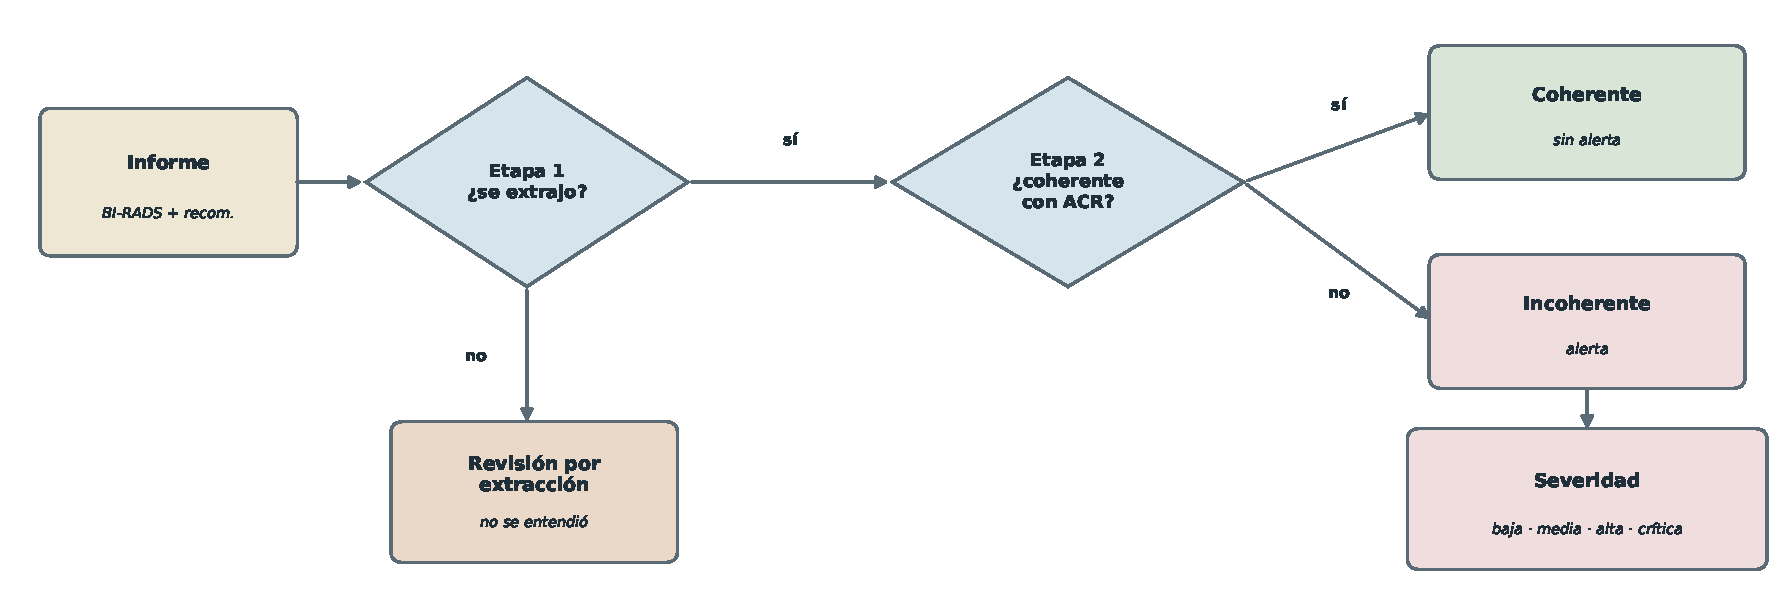
\includegraphics[width=0.92\textwidth]{figuras/fig_arq_cotejo.pdf}
\caption{C\'omo el sistema decide sobre un informe. En la Etapa~1 verifica si pudo entender el informe; si no, lo deriva a revisi\'on por extracci\'on. En la Etapa~2 la auditor\'ia es binaria: la recomendaci\'on es coherente (coincide, equivale o es m\'as cauta) o incoherente. Toda incoherencia genera alerta, graduada de baja a cr\'itica seg\'un su impacto en salud.}
\label{fig:cotejo}
\end{figure*}

\paragraph{Graduaci\'on de la alerta por impacto en salud}
La auditor\'ia de coherencia es binaria: una recomendaci\'on es coherente o no lo es. Es coherente cuando coincide con la esperada, es un equivalente aceptable, o es m\'as cauta que la m\'inima esperada, ya que un exceso de precauci\'on --por ejemplo, biopsiar un BI-RADS 3-- es cl\'inicamente v\'alido. Es incoherente cuando la recomendaci\'on se queda corta frente a la norma. Toda incoherencia genera una alerta; lo que var\'ia es su severidad, no el hecho de constituir o no un problema. As\'i, la palabra alerta conserva su significado, y su gravedad, desde una incoherencia leve y sin riesgo hasta una cr\'itica, comunica cu\'anto importa.

La severidad no proviene de casos particulares del corpus, sino de una regla general que combina dos factores medibles para cualquier informe: la criticidad del BI-RADS, que la norma ACR fija de antemano (BI-RADS 4 y 5 conllevan sospecha de malignidad; 0 y 6 son intermedios; 1, 2 y 3 son de bajo riesgo), y cu\'anto se aparta la recomendaci\'on de la conducta esperada dentro de la jerarqu\'ia de urgencia. La regla central, validada con criterio cl\'inico, es que una sospecha de malignidad (BI-RADS 4 o 5) cuya recomendaci\'on no incluya biopsia ni derivaci\'on se clasifica siempre como cr\'itica, pues cualquier conducta que no confirme el diagn\'ostico implica un riesgo de retraso. Una incoherencia leve, en cambio, corresponde a un desv\'io menor en una categor\'ia de bajo riesgo, sin consecuencias para la paciente. La Tabla~\ref{tab:niveles} resume los desenlaces y su distribuci\'on en el corpus.

A este esquema se suma un desenlace de naturaleza distinta. Cuando el sistema no logra extraer ni clasificar la recomendaci\'on, no puede juzgar la coherencia, de modo que no afirma que el caso sea correcto ni inventa una inconsistencia: lo marca como revisi\'on por extracci\'on y lo deriva a un humano. Esta abstenci\'on es deliberada. Distingue con honestidad los casos en que el sistema entendi\'o el informe y hall\'o un desacuerdo cl\'inico de aquellos en que sencillamente no pudo leerlo, quiz\'a por un formato at\'ipico.

La severidad de esa revisi\'on depende de la categor\'ia. Cuando el BI-RADS es 4, 5 o 6, la ausencia de una recomendaci\'on clasificable se marca como cr\'itica. La norma ACR exige una conducta expl\'icita para esas categor\'ias, de modo que su ausencia en el informe no es un problema t\'ecnico de lectura sino un vac\'io de documentaci\'on en el escenario de mayor riesgo. Es la contraparte de la alerta de omisi\'on del M\'odulo~1: all\'i falta la categor\'ia, aqu\'i falta la conducta. Para el resto de las categor\'ias la revisi\'on se marca con prioridad media.

\begin{table}[!t]
\caption{Desenlaces del cotejo y su distribuci\'on en el corpus (4\,357 informes). La auditor\'ia es binaria (coherente o incoherente); la incoherencia se grad\'ua de baja a cr\'itica. En total, 50 informes (1,1\,\%) resultan incoherentes.}
\label{tab:niveles}
\centering
\footnotesize
\begin{tabular}{@{}p{0.26\columnwidth}p{0.51\columnwidth}r@{}}
\toprule
\textbf{Desenlace} & \textbf{Situaci\'on} & \textbf{Casos} \\
\midrule
Coherente & Coincide, equivale o es m\'as cauta (sin alerta) & 4\,299 \\
Incoh.\ cr\'itica & Sospecha (BI-RADS 4/5) sin acci\'on diagn\'ostica & 19 \\
Incoh.\ alta & Desv\'io relevante en categor\'ia intermedia & 18 \\
Incoh.\ media & Inconsistencia a revisar, sin urgencia & 9 \\
Incoh.\ baja & Desv\'io menor sin riesgo para la paciente & 4 \\
Revisi\'on ext. & No se pudo extraer o clasificar la recomendaci\'on & 8 \\
\bottomrule
\end{tabular}
\end{table}

\subsubsection{M\'odulo 4: verificador del BI-RADS, dise\~nado y retirado (\codename{verificador\_birads\_ml.py})}
Este m\'odulo se plante\'o para obtener la categor\'ia por dos v\'ias y contrastarlas: la extracci\'on por reglas del M\'odulo~1 y un DistilBETO que relee el mismo texto. Priorizaba la regla, bajo el supuesto de que la categor\'ia escrita por el radi\'ologo es la referencia, y reservaba la voz del modelo para los casos de baja confianza, distinguiendo cinco estados seg\'un el acuerdo entre ambas (Fig.~\ref{fig:estados}). El modelo lee una ventana local alrededor de la menci\'on candidata para que ambas v\'ias trabajen sobre el mismo fragmento.

Se implement\'o y se evalu\'o por completo, y la evaluaci\'on llev\'o a retirarlo: la Secci\'on~\ref{sec:verif} detalla las mediciones. El M\'odulo~1 opera solo con reglas (\codename{usar\_verificador\_ml=False}). El c\'odigo se conserva en el repositorio junto con su evaluaci\'on, dado que el resultado negativo delimita el rol de la IA en el sistema.

\subsection{Arquitectura del pipeline}
Un informe textual ingresa al pipeline y atraviesa los cuatro m\'odulos en secuencia. El programa opera as\'i: primero recibe el texto del informe; el M\'odulo~1 localiza y extrae la categor\'ia BI-RADS declarada; el M\'odulo~2 localiza el texto de la recomendaci\'on, primero por su encabezado y, si el informe no lo tiene, mediante un \emph{fallback} que recorre el texto buscando frases gatillo de conducta, de modo que la extracci\'on no dependa de una estructura fija, y luego lo clasifica en una de ocho categor\'ias cl\'inicas; el M\'odulo~3 consulta la tabla normativa BI-RADS/ACR y contrasta la recomendaci\'on clasificada con la esperada para esa categor\'ia, emitiendo un estado de coherencia y, si corresponde, una alerta con su severidad. Cuando el M\'odulo~2 no logra clasificar con confianza, la recomendaci\'on se marca como \emph{ambigua} y se deriva a revisi\'on humana en vez de forzar una categor\'ia.

El pipeline produce una salida estructurada y trazable, con la categor\'ia BI-RADS extra\'ida y su nivel de confianza, la recomendaci\'on clasificada y la esperada, el estado del cotejo, un mensaje explicativo y la regla aplicada. Cada uno de estos campos queda accesible para auditor\'ia, en coherencia con la filosof\'ia Human-on-the-Loop.

\subsection{M\'etricas de evaluaci\'on}
La evaluaci\'on se realiz\'o sobre el corpus completo (4\,357 informes) utilizando: (i) \emph{accuracy} y \emph{Macro F1} para la extracci\'on de BI-RADS y para la predicci\'on del modelo ML, reportadas bajo split \'unico estratificado y bajo validaci\'on cruzada 5-fold estratificada; (ii) \emph{cobertura} (\% de informes con recomendaci\'on clasificada) para el m\'odulo 2; (iii) \emph{tasa de alertas cl\'inicas} (\% del corpus que genera alerta) como indicador de fatiga de alertas; (iv) \emph{cobertura de variantes de formato} sobre la bater\'ia de casos sint\'eticos. Para el m\'odulo~4, evaluado y luego retirado, se reportan adem\'as la ca\'ida bajo ablaci\'on y la comparaci\'on contra una l\'inea base trivial, que son las mediciones que motivaron su descarte.

\subsection{Implementaci\'on}
El sistema se implement\'o en Python 3.9, con \texttt{transformers 4.57.6}, \texttt{torch 2.8.0}, y \texttt{scikit-learn 1.6.1}. La aceleraci\'on por hardware utiliz\'o Metal Performance Shaders (MPS) de Apple Silicon. El c\'odigo es p\'ublico bajo el repositorio \texttt{proyecto-ia-mamografia}\footnote{\url{https://github.com/SebasDCIS/proyecto-ia-mamografia}}, organizado en m\'odulos \texttt{src/} con tests inline y notebooks de exploraci\'on \texttt{notebooks/05} a \texttt{10}. La reproducibilidad est\'a garantizada mediante \texttt{requirements.txt} y semillas fijas (\texttt{numpy}, \texttt{torch}, \texttt{random}) en los splits estratificados y en cada fold de la validaci\'on cruzada.

\subsection{Interfaz de visualizaci\'on}
Para acercar el sistema al usuario cl\'inico se desarroll\'o una interfaz web ligera (Fig.~\ref{fig:dashboard}). El usuario pega el texto de un informe y obtiene, de inmediato, el desenlace del cotejo comunicado en t\'erminos simples: la categor\'ia BI-RADS extra\'ida, la recomendaci\'on detectada, la esperada por el est\'andar, y un distintivo de color que resume el resultado: coherente, incoherente (con su severidad) o revisi\'on por extracci\'on. La interfaz privilegia la legibilidad para un profesional no t\'ecnico: muestra un mensaje explicativo en lenguaje cl\'inico, y ofrece la trazabilidad de la regla aplicada en un panel desplegable para quien desee auditar la decisi\'on. Toda la ejecuci\'on ocurre localmente, en coherencia con los requisitos de privacidad del sistema.

\begin{figure}[!t]
\centering
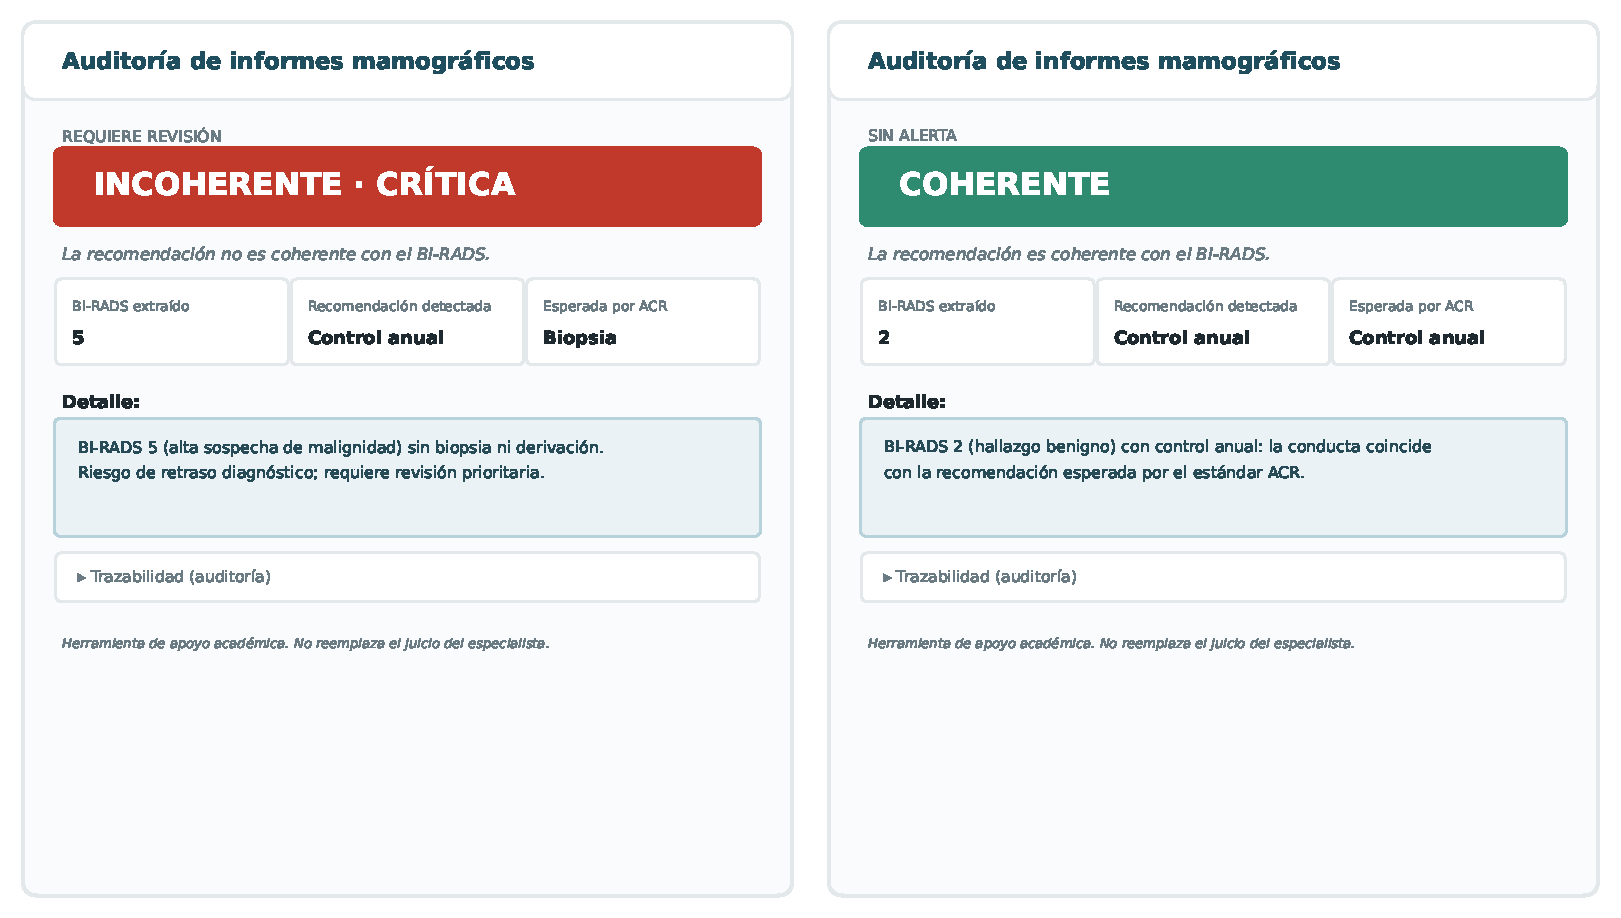
\includegraphics[width=\columnwidth]{figuras/fig_dashboard.pdf}
\caption{Interfaz de auditor\'ia sobre dos informes de ejemplo. A la izquierda, una alerta cr\'itica (BI-RADS 5 con control anual); a la derecha, un caso coherente sin alerta (BI-RADS 2 con control anual). Cada resultado muestra el BI-RADS, la recomendaci\'on detectada y la esperada, junto con un mensaje explicativo.}
\label{fig:dashboard}
\end{figure}

\section{Resultados y Discusi\'on}

\subsection{M\'etricas de desempe\~no}\label{sec:metricas-desempeno}
La Tabla~\ref{tab:modulos} resume el desempe\~no de los m\'odulos sobre el corpus completo. La extracci\'on de BI-RADS por reglas alcanz\'o Macro F1 = 0,9995 (exactitud 99,9\%) con cobertura total, confirmando que la localizaci\'on de la categor\'ia declarada es una tarea esencialmente reglada. El extractor de recomendaciones clasific\'o el 99,8\% del corpus mediante reglas cl\'inicas con confianza alta. El extractor NER de respaldo alcanz\'o un F1 a nivel de span de 0,999 en el conjunto de prueba deduplicado; como se discute m\'as adelante, esta cifra refleja la homogeneidad del corpus m\'as que la generalizaci\'on, por lo que su valor real se evalu\'o con informes externos. El motor de cotejo BI-RADS/ACR gener\'o alerta cl\'inica en solo el 1,15\% de los informes, un nivel bajo de fatiga de alertas.

Para el clasificador Transformer, la Tabla~\ref{tab:folds} detalla los resultados por fold de la validaci\'on cruzada. Su Macro F1 es 0,8877 $\pm$ 0,0501, por encima del mejor baseline cl\'asico (LinearSVC, 0,7369 $\pm$ 0,0703; Fig.~\ref{fig:comparacion}). Ese resultado motiv\'o en su momento adoptarlo, y la Secci\'on~\ref{sec:verif} explica por qu\'e se retir\'o despu\'es.

\begin{table}[!t]
\caption{Desempe\~no por m\'odulo sobre el corpus completo (4\,357 informes).}
\label{tab:modulos}
\centering
\footnotesize
\begin{tabular}{@{}lll@{}}
\toprule
M\'odulo & M\'etrica & Valor \\
\midrule
Extracci\'on BI-RADS (regex) & Macro F1 / cobertura & 0,9995 / 100\% \\
Clasificaci\'on recomendaci\'on & cobertura (reglas) & 99,82\% \\
Extractor NER recomendaci\'on & F1 span (test dedup.) & 0,999 \\
Cotejo BI-RADS/ACR & tasa de incoherencias & 1,15\% \\
Verificador DistilBETO \emph{(descartado)} & Macro F1 (CV 5-fold) & 0,8877 $\pm$ 0,0501 \\
\bottomrule
\end{tabular}
\end{table}

\begin{table}[!t]
\caption{Resultados por fold de la validaci\'on cruzada estratificada 5-fold de DistilBETO con aumentaci\'on aplicada por fold.}
\label{tab:folds}
\centering
\footnotesize
\begin{tabular}{@{}cccc@{}}
\toprule
Fold & Accuracy & Macro F1 & Weighted F1 \\
\midrule
1 & 0,9851 & 0,9113 & 0,9849 \\
2 & 0,9874 & 0,9262 & 0,9875 \\
3 & 0,9874 & 0,8842 & 0,9872 \\
4 & 0,9805 & 0,8024 & 0,9800 \\
5 & 0,9816 & 0,9144 & 0,9817 \\
\midrule
Media & 0,9844 & \textbf{0,8877} & 0,9852 \\
$\sigma$ & 0,0032 & 0,0501 & 0,0032 \\
\bottomrule
\end{tabular}
\end{table}

\begin{figure}[!t]
\centering
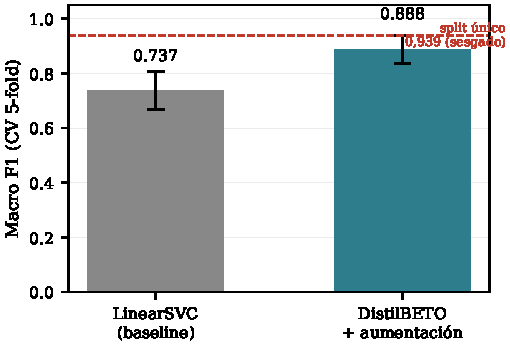
\includegraphics[width=0.9\columnwidth]{figuras/fig_comparacion_modelos.pdf}
\caption{Macro F1 bajo validaci\'on cruzada 5-fold. DistilBETO supera al baseline LinearSVC con margen robusto. La l\'inea punteada marca el Macro F1 del split \'unico (0,939), optimista por el sesgo de selecci\'on de checkpoint.}
\label{fig:comparacion}
\end{figure}

\subsection{Comparaci\'on con trabajos previos}\label{sec:comparacion}
Los trabajos citados en la Secci\'on~\ref{sec:intro} permiten situar estos resultados, con una precauci\'on: no todos abordan la misma tarea.

Sippo \emph{et al.}~\cite{sippo2013} extraen la categor\'ia BI-RADS de informes en ingl\'es mediante expresiones regulares y reportan 100\,\% de \emph{recall} y 96,6\,\% de precisi\'on. Es la referencia m\'as directa, porque resuelve la misma tarea de localizar un dato declarado. El extractor descrito aqu\'i alcanza Macro F1 = 0,9995 sobre 4\,357 informes en espa\~nol. La comparaci\'on tiene sentido en cuanto al enfoque, aunque los corpus difieren en idioma, origen y estructura, de modo que las cifras no son intercambiables.

L\'opez-\'Ubeda \emph{et al.}~\cite{lopez2024} reportan Macro F1 = 0,74 con BETO sobre un corpus espa\~nol peninsular. Esa cifra corresponde a \emph{predecir} la categor\'ia a partir del texto, no a extraer la que el radi\'ologo declar\'o, y por eso no debe contrastarse con el 0,9995 de la v\'ia reglada. El experimento equivalente en este trabajo es la predicci\'on del BI-RADS desde los hallazgos, que alcanza Macro F1 = 0,624 fuera de fold. La diferencia entre ambos valores se explica por la disponibilidad de datos en las clases cr\'iticas: en el corpus utilizado, las categor\'ias 4, 5 y 6 re\'unen 52, 16 y 5 ejemplos respectivamente.

Confundir esas dos tareas es el error que este trabajo procura evitar. Una regla que localiza una cadena declarada y un modelo que infiere una categor\'ia desde los hallazgos resuelven problemas distintos, y sus m\'etricas no son comparables aunque compartan el nombre de la etiqueta. La auditor\'ia de coherencia requiere la primera, no la segunda.

Kuling \emph{et al.}~\cite{kuling2022} atacan un problema adyacente, la segmentaci\'on de secciones del informe, con 98\,\% de acierto. Ese componente es an\'alogo al M\'odulo~0 de este sistema, aunque aqu\'i se resuelve por reglas y no por un modelo, y sin m\'etrica propia porque su efecto se observa aguas abajo.

La diferencia de fondo con los tres trabajos es de objetivo. Todos abordan la extracci\'on o clasificaci\'on de la categor\'ia BI-RADS; ninguno coteja esa categor\'ia contra la recomendaci\'on cl\'inica para detectar incoherencias, que es el aporte de este sistema y la raz\'on por la que la tabla normativa del M\'odulo~3 no tiene equivalente en la literatura revisada.

\subsection{Estudio descriptivo de los datos}
La Fig.~\ref{fig:distbirads} muestra la marcada asimetr\'ia de clases del corpus: BI-RADS 2 concentra el 60,5\% de los informes, mientras que las categor\'ias cl\'inicamente cr\'iticas son minoritarias (BI-RADS 4, 5 y 6 suman apenas el 1,7\%). Esta distribuci\'on justifica dos decisiones metodol\'ogicas centrales: el uso de Macro F1 --que pondera por igual todas las clases-- en lugar de \emph{accuracy}, que quedar\'ia dominada por la clase mayoritaria; y la aplicaci\'on de aumentaci\'on textual dirigida a las clases minoritarias durante el entrenamiento del Transformer.

La Fig.~\ref{fig:distrec} presenta la distribuci\'on de las recomendaciones clasificadas por el m\'odulo 2. Predominan la correlaci\'on ecogr\'afica (45,9\%) y el control anual (29,6\%), coherente con la alta prevalencia de BI-RADS 0 y 2; la escasez de recomendaciones de biopsia (1,4\%) refleja la baja frecuencia de las categor\'ias sospechosas y refuerza el desaf\'io de clasificar correctamente dichas clases.

\begin{figure}[!t]
\centering
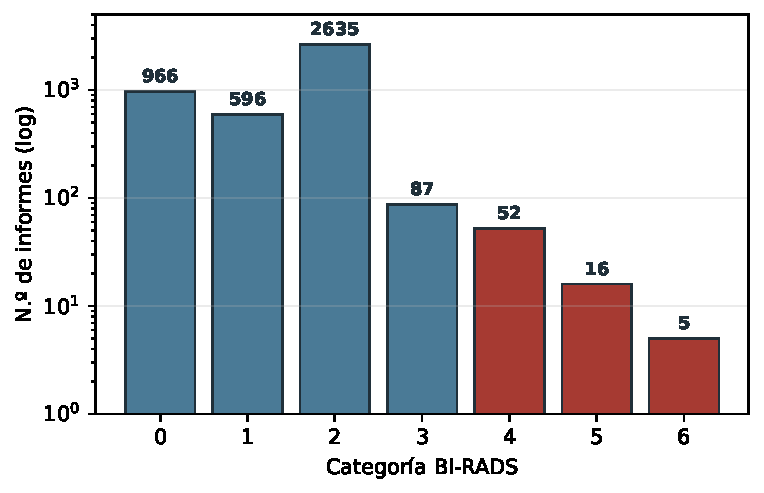
\includegraphics[width=0.9\columnwidth]{figuras/fig_distribucion_birads.pdf}
\caption{Distribuci\'on de categor\'ias BI-RADS en el corpus (escala logar\'itmica). El fuerte desbalance --BI-RADS 2 concentra el 60,5\%; las clases cr\'iticas 4/5/6 el 1,7\%-- motiva el uso de Macro F1 y la aumentaci\'on de clases minoritarias.}
\label{fig:distbirads}
\end{figure}

\begin{figure}[!t]
\centering
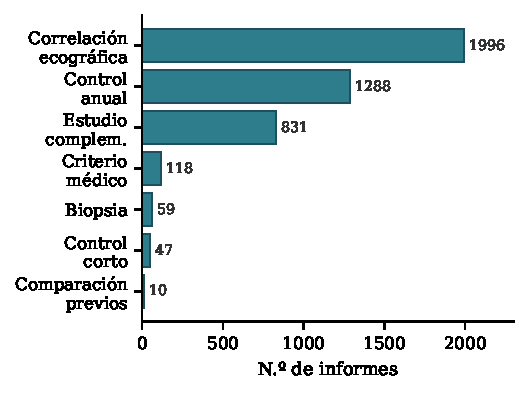
\includegraphics[width=0.9\columnwidth]{figuras/fig_distribucion_recomendaciones.pdf}
\caption{Distribuci\'on de las categor\'ias de recomendaci\'on clasificadas por el m\'odulo 2 sobre el corpus.}
\label{fig:distrec}
\end{figure}

\subsection{An\'alisis de resultados del pipeline}

\subsubsection{El verificador Transformer: por qu\'e se retir\'o}
El M\'odulo~4 se dise\~n\'o como verificaci\'on cruzada de la extracci\'on reglada y se retir\'o tras medirlo. Dos resultados lo determinan.

El estudio de ablaci\'on (Fig.~\ref{fig:ablacion}) enmascara la menci\'on textual del n\'umero BI-RADS y reeval\'ua: el Macro F1 cae de 0,9386 a 0,5438, un 42\,\% menos. El modelo lee la categor\'ia declarada en lugar de deducirla de los hallazgos.

La comparaci\'on contra una l\'inea base trivial cierra el punto. En inferencia el modelo recibe una ventana de 250 caracteres centrada en la menci\'on que la regla seleccion\'o. Sobre esa misma ventana, una expresi\'on regular de una l\'inea alcanza 99,82\,\% de exactitud y DistilBETO 99,78\,\%. Ambas v\'ias leen la misma cadena, de modo que el contraste entre ellas no constituye una segunda opini\'on independiente sino una relectura del mismo dato.

La causa de fondo es que leer una categor\'ia declarada no admite discrepancia informativa: \codename{BI-RADS 4} no es ambiguo. Un segundo lector aportar\'ia si dedujera la categor\'ia desde los hallazgos, tarea que se evalu\'o por separado y alcanza Macro F1 = 0,624 fuera de fold, insuficiente en las clases cr\'iticas. El M\'odulo~1 opera en consecuencia solo con reglas, con Macro F1 = 0,9995. La IA se mantiene donde la evaluaci\'on respalda su uso, el extractor NER del M\'odulo~2, cuya tarea presenta variaci\'on sem\'antica y no tipogr\'afica: los formatos de un n\'umero se enumeran en una tabla; las redacciones de una recomendaci\'on cl\'inica, no.

La Fig.~\ref{fig:estados} resume la salida que produc\'ia el verificador: el 96,4\% de los informes result\'o \emph{confirmado} (regex de alta confianza y ML concordante), un 3,0\% obtuvo \emph{confirmaci\'on cruzada} (regex de menor confianza respaldada por el ML), un 0,6\% qued\'o sin confirmaci\'on del ML (prevaleciendo la regex), y solo un 0,07\% constituy\'o una discrepancia real que amerita revisi\'on manual. Esa concordancia casi total no mide acierto sino redundancia: el modelo relee la cadena que la regla ya extrajo, de modo que coincidir es el resultado esperable.

\begin{figure}[!t]
\centering
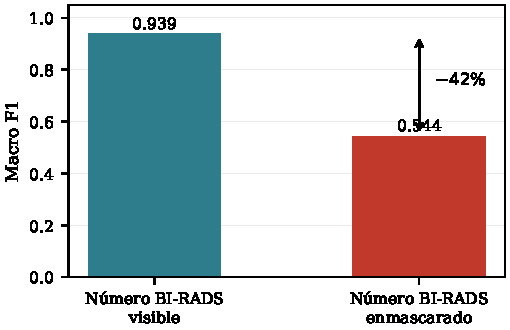
\includegraphics[width=0.9\columnwidth]{figuras/fig_ablacion.pdf}
\caption{Estudio de ablaci\'on. Al enmascarar el n\'umero BI-RADS del texto, el Macro F1 del Transformer cae un 42\% (0,939 $\rightarrow$ 0,544), evidenciando que el modelo lee la categor\'ia declarada m\'as que deducirla de los hallazgos.}
\label{fig:ablacion}
\end{figure}

\begin{figure}[!t]
\centering
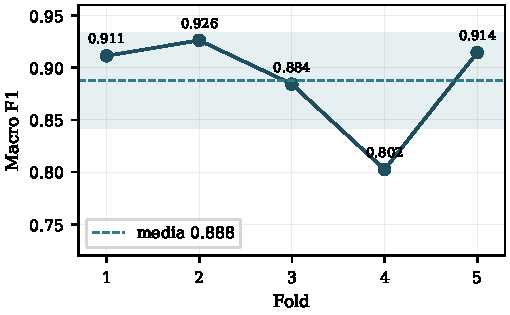
\includegraphics[width=0.9\columnwidth]{figuras/fig_variabilidad_folds.pdf}
\caption{Macro F1 por fold en la validaci\'on cruzada. La ca\'ida del fold 4 (0,80) refleja la sensibilidad de la m\'etrica macro a las clases minoritarias y justifica reportar la CV en lugar de un split \'unico.}
\label{fig:folds}
\end{figure}

\begin{figure}[!t]
\centering
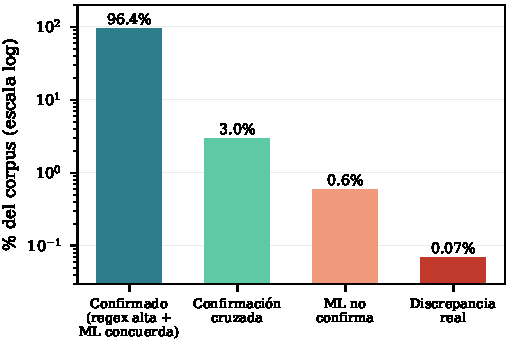
\includegraphics[width=0.9\columnwidth]{figuras/fig_estados_verificacion.pdf}
\caption{Distribuci\'on de estados del verificador Transformer que se dise\~n\'o y luego se retir\'o. El 96,4\,\% de los informes queda confirmado y solo el 0,07\,\% produce una discrepancia real. Esa concordancia casi total es consecuencia de que el modelo relee la misma cadena que la regla ya extrajo, y es una de las cuatro evidencias que motivaron el descarte (Secci\'on~\ref{sec:verif}).}
\label{fig:estados}
\end{figure}

\subsection{Extractor NER de recomendaciones: desempe\~no y generalizaci\'on}
El extractor neuronal se entren\'o sobre el corpus con etiquetas derivadas autom\'aticamente, previa deduplicaci\'on robusta para evitar fuga de informaci\'on entre particiones. La Tabla~\ref{tab:hiperparametros} detalla los hiperpar\'ametros de este entrenamiento y los del verificador que se descart\'o, ambos afinados a partir de DistilBETO. Para el NER se cuid\'o especialmente evitar el sobreajuste y la fuga: el conjunto se separ\'o en entrenamiento, validaci\'on y prueba antes de tokenizar; se aplic\'o \emph{early stopping} guiado solo por la validaci\'on; y la longitud m\'axima de secuencia se fij\'o en 384 subtokens para no truncar la recomendaci\'on, que suele ubicarse al final del informe.

En el conjunto de prueba deduplicado alcanz\'o un F1 a nivel de span de 0,999 (Fig.~\ref{fig:ner}). Esta cifra debe leerse con cautela. El corpus es muy homog\'eneo: la recomendaci\'on aparece siempre al final del informe y, tras normalizar el texto, existen apenas 221 recomendaciones distintas (la m\'as frecuente se repite 784 veces), de modo que el valor mide la facilidad del corpus y no la capacidad de generalizar. La evaluaci\'on relevante se hizo entonces sobre informes chilenos externos, de formato no visto. All\'i el modelo extrajo correctamente redacciones que las reglas no cubr\'ian, como \emph{``complementar examen con ecograf\'ia''}, y cuando el informe no tra\'ia recomendaci\'on expl\'icita no extrajo nada, sin inventar texto. El desempe\~no dentro del corpus y el comportamiento en datos externos difieren, y esa diferencia orienta la mejora de fondo hacia un corpus del contexto de despliegue. Mientras tanto, el NER cumple un rol acotado de respaldo, con las reglas transparentes como v\'ia primaria.

\begin{table}[!t]
\caption{Hiperpar\'ametros de los dos entrenamientos afinados sobre DistilBETO.}
\label{tab:hiperparametros}
\centering
\footnotesize
\begin{tabular}{@{}lll@{}}
\toprule
Hiperpar\'ametro & Verificador BI-RADS & Extractor NER \\
\midrule
Tarea & clasificaci\'on sec. & etiquetado (NER) \\
Modelo base & DistilBETO & DistilBETO \\
\'Epocas & 3 & 6 (early stop.) \\
Batch size & 8 & 16 \\
Learning rate & $2\times10^{-5}$ & $3\times10^{-5}$ \\
Weight decay & 0,01 & 0,01 \\
Warmup ratio & sin configurar (0) & 0,1 \\
Long. m\'ax. (subtokens) & 256 & 384 \\
Selecci\'on de modelo & CV 5-fold & mejor F1 val. \\
Partici\'on & CV estratif. & 70/15/15 estratif. \\
Semilla & fija & 42 \\
\bottomrule
\end{tabular}
\end{table}

\begin{figure}[!t]
\centering
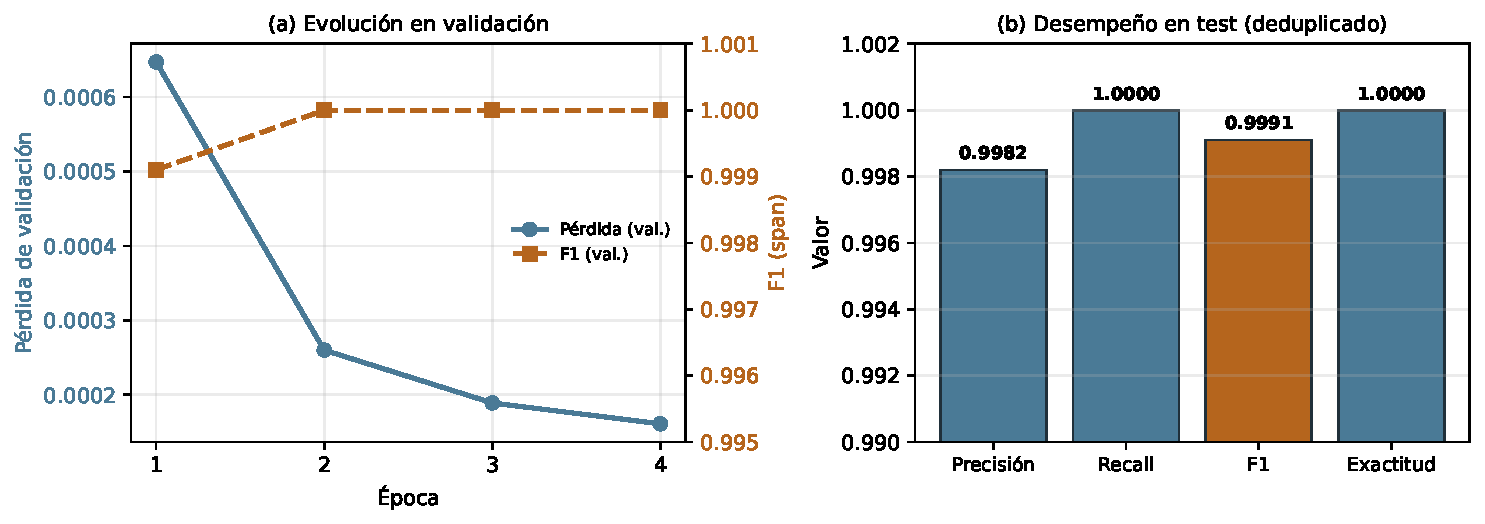
\includegraphics[width=\columnwidth]{figuras/fig_ner_entrenamiento.pdf}
\caption{Entrenamiento y desempe\~no del extractor NER. (a) La p\'erdida de validaci\'on desciende y el F1 se estabiliza en pocas \'epocas; el \emph{early stopping} carga el mejor modelo. (b) M\'etricas a nivel de span en el conjunto de prueba deduplicado. Los valores cercanos a la unidad reflejan la homogeneidad del corpus; la evaluaci\'on de generalizaci\'on se hizo con informes externos.}
\label{fig:ner}
\end{figure}

\subsubsection{Prueba de estr\'es: redacciones no anticipadas}\label{sec:estres}
El F1 de 0,9991 mide el NER dentro del corpus, pero su rol es servir de respaldo ante redacciones que las reglas no anticiparon, y ese rol se ejerce fuera del corpus. La m\'etrica del corpus no lo eval\'ua. De hecho, medido dentro, una expresi\'on regular que localiza el \'ultimo verbo gatillo y marca hasta el final del informe alcanza F1 = 0,9991 frente al 1,0000 del NER: sobre este corpus el modelo no aporta, porque el 98,1\,\% de las recomendaciones comienza con la misma f\'ormula y todas ocupan la posici\'on final.

La evidencia a favor del NER son los tres informes chilenos donde las reglas fallaron, lo que es poco. Para medir su rol sobre una muestra mayor se perturb\'o el conjunto de prueba de modo que reprodujera la brecha: se elimin\'o el encabezado \codename{RECOMENDACIONES} y se sustituy\'o el verbo gatillo por formas verificadas como ausentes de \codename{\_FRASES\_GATILLO\_RECOMENDACION}, la lista cerrada del m\'odulo. Los reemplazos se comprobaron uno a uno contra esa expresi\'on regular y todos tienen dos tokens, de modo que el span conserva su posici\'on y su largo. La regla evaluada es el m\'odulo de producci\'on en su segunda v\'ia, la que opera cuando no existe columna de recomendaciones, es decir la que se ejecuta ante un PDF.

\begin{table}[!t]
\caption{Prueba de estr\'es sobre 565 informes de prueba: F1 de span exacto.}
\label{tab:estres}
\centering
\begin{tabular}{@{}lcc@{}}
\toprule
\textbf{Condici\'on} & \textbf{Regla} & \textbf{NER} \\
\midrule
Control & 1,0000 & 1,0000 \\
Sin encabezado & 0,9460 & 1,0000 \\
Verbo fuera de la lista & 1,0000 & 0,9929 \\
\textbf{Sin encabezado y verbo nuevo} & \textbf{0,5314} & \textbf{0,9956} \\
\bottomrule
\end{tabular}
\end{table}

La Tabla~\ref{tab:estres} muestra que la regla dispone de dos se\~nales independientes y se sostiene mientras conserve una de ellas: sin encabezado alcanza 0,9460 porque el verbo la rescata, y con un verbo desconocido alcanza 1,0000 porque el encabezado la rescata. Al retirar ambas queda en 0,5314. El NER no depende de ninguna de las dos y se mantiene entre 0,9929 y 1,0000 en las cuatro condiciones.

La \'ultima fila es la que corresponde al caso chileno: un informe sin encabezado expl\'icito y con una redacci\'on no prevista. Ah\'i la regla pierde cerca de la mitad de las recomendaciones y el NER conserva 0,9956. Ese resultado delimita el aporte del modelo: no mejora la extracci\'on en el corpus, donde una regla trivial lo iguala, sino que sostiene el desempe\~no cuando las se\~nales que las reglas presuponen no est\'an.

El contraste con el verificador de BI-RADS resulta expl\'icito bajo la misma prueba. Al enmascarar la se\~nal de la que depende cada modelo, el verificador cae de 0,939 a 0,544 mientras que el NER pasa de 1,000 a 0,9956. El verificador dispon\'ia de una sola se\~nal, el n\'umero declarado, y sin ella no le quedaba nada que leer. El NER aprendi\'o a reconocer qu\'e constituye una recomendaci\'on cl\'inica en lugar de memorizar los t\'erminos que la introducen.

Este experimento es sint\'etico: opera sobre el corpus paraguayo perturbado y no sobre informes chilenos reales. Mide el rol que el componente cumple, no su desempe\~no en Chile. La validaci\'on con un corpus chileno anotado sigue siendo la limitaci\'on de fondo del trabajo.

\subsection{Cobertura ante variantes de formato}\label{sec:robustez}
El corpus de entrenamiento es homog\'eneo. Todos sus informes traen encabezado de conclusi\'on, ninguno escribe la categor\'ia con numerales romanos, la recomendaci\'on ocupa siempre la posici\'on final y los datos del paciente ya vienen retirados. Esa uniformidad permite que un sistema sostenga supuestos sin que nada los ponga a prueba, y fue el origen de varias fragilidades descritas en las secciones anteriores.

Para verificar la cobertura sobre variantes que el corpus no contiene se construy\'o una bater\'ia de 16 casos de prueba sint\'eticos. Son informes ficticios, con nombres, identificadores y fechas inventados, que reproducen formas de redacci\'on y estructura documentadas en la pr\'actica cl\'inica local. Cada caso declara el resultado esperado, de modo que la bater\'ia funciona tambi\'en como prueba de regresi\'on y puede ejecutarse sin acceso a datos cl\'inicos.

\begin{table}[!t]
\caption{Bater\'ia de casos sint\'eticos: variantes cubiertas.}
\label{tab:formatos}
\centering
\begin{tabular}{@{}p{2.3cm}p{5.4cm}@{}}
\toprule
\textbf{Grupo} & \textbf{Variantes} \\
\midrule
Escritura del BI-RADS & Ar\'abigo; numeral romano (\emph{Birads -us III}); modalidad antepuesta (\emph{US BIRADS 1}) y pospuesta (\emph{Birads 2 US}); error de tipeo (\emph{bi-radas}) \\
Estructura & \emph{Impresi\'on mamogr\'afica} en lugar de \emph{Conclusi\'on}; sin encabezado; descargo legal reubicado al inicio; menci\'on hist\'orica previa a la definitiva \\
Recomendaci\'on & Forma verbal (\emph{controlar} por \emph{control}); sin\'onimos de t\'ecnica (\emph{ultrasonido}) \\
Comportamiento seguro & Hallazgos sin categor\'ia; sospecha sin conducta declarada; incoherencia cr\'itica \\
Privacidad & Nombre e identificador adheridos al texto cl\'inico \\
\bottomrule
\end{tabular}
\end{table}

El sistema resuelve correctamente los 16 casos en las cuatro dimensiones evaluadas: categor\'ia extra\'ida, recomendaci\'on clasificada, estado del cotejo y ausencia de identificadores tras la limpieza. La Tabla~\ref{tab:formatos} resume los grupos cubiertos.

Dos resultados merecen comentario. El primero es que el corpus no contiene ni un solo numeral romano, mientras que la pr\'actica local s\'i los emplea. El soporte para esa variante se program\'o como cobertura preventiva, sin disponer de un ejemplo que lo justificara, y la bater\'ia lo verifica. Un modelo entrenado sobre el corpus no podr\'ia cubrirla, porque nunca la vio: es un argumento concreto a favor de las reglas en una tarea donde la variaci\'on es tipogr\'afica y enumerable.

El segundo es el caso de una categor\'ia de alta sospecha que no declara ninguna conducta. Ese escenario motiv\'o el escalamiento de severidad descrito en el M\'odulo~3. Sin \'el, la ausencia de recomendaci\'on en un BI-RADS 5 se habr\'ia tratado igual que en un BI-RADS 1.

La bater\'ia verifica cobertura de formatos, no desempe\~no poblacional. Los casos son sint\'eticos y construidos para cubrir variantes conocidas, de modo que no sustituyen la validaci\'on con un corpus cl\'inico anotado del contexto de despliegue, que sigue siendo la limitaci\'on de fondo del trabajo. Lo que s\'i permiten es distinguir entre un sistema que funciona sobre su corpus y uno que funciona sobre las formas en que los informes se escriben en la pr\'actica.

\subsection{Verificaci\'on de las decisiones de dise\~no}\label{sec:verif}
La elecci\'on de un n\'ucleo reglado se someti\'o a verificaci\'on emp\'irica en lugar de asumirse. Se dise\~n\'o una serie de experimentos controlados para contrastar, sobre la misma tarea y corpus, el enfoque reglado frente a alternativas basadas en aprendizaje autom\'atico, con el fin de fundamentar la arquitectura final en evidencia.

Primero, cuatro pruebas independientes sobre el verificador Transformer (ablaci\'on, frecuencia de intervenci\'on, comparaci\'on contra una l\'inea base trivial y recuperaci\'on de formatos no vistos) mostraron que no aporta sobre la v\'ia reglada, lo que llev\'o a retirarlo del pipeline. Segundo, se verific\'o el l\'imite de una l\'inea de \emph{predicci\'on} del BI-RADS desde los hallazgos, cuyo desempe\~no queda determinado por la disponibilidad de datos en las clases cl\'inicamente cr\'iticas --una propiedad del corpus, no de la t\'ecnica--, lo que orienta el trabajo futuro hacia la recolecci\'on de datos. Tercero, se evaluaron enfoques de \emph{embeddings} sem\'anticos como refuerzo de la clasificaci\'on de recomendaciones; la evaluaci\'on mostr\'o que el enfoque reglado captura mejor la jerarqu\'ia cl\'inica de las recomendaciones compuestas, consolidando su elecci\'on como m\'etodo principal.

La convergencia de estos experimentos aporta un respaldo s\'olido a la arquitectura: para una tarea de granularidad cl\'inica fina, sobre un corpus con fuerte desbalance, y en un dominio que exige transparencia, reproducibilidad, auditabilidad y ejecuci\'on local, el enfoque reglado es la opci\'on m\'as adecuada, y el aprendizaje autom\'atico se reserva para roles acotados y verificados. Esta verificaci\'on metodol\'ogica constituye una de las contribuciones del trabajo.

\subsection{Limitaciones}\label{sec:limitaciones}
El trabajo tiene cuatro limitaciones que conviene declarar de forma expl\'icita.

\textbf{Origen del corpus.} Los 4\,357 informes son de origen paraguayo, mientras que el contexto de despliegue previsto es chileno. El corpus es adem\'as homog\'eneo: todos sus informes traen encabezado de conclusi\'on, ninguno escribe la categor\'ia con numerales romanos y los datos del paciente ya vienen retirados. Esa uniformidad permite sostener supuestos que la pr\'actica local no respeta, y fue el origen de varias fragilidades corregidas durante el desarrollo. La bater\'ia de casos sint\'eticos de la Secci\'on~\ref{sec:robustez} verifica cobertura de formatos, no desempe\~no poblacional, y no sustituye la validaci\'on con un corpus cl\'inico anotado del contexto de despliegue.

\textbf{Validaci\'on cl\'inica de la tabla normativa.} La formalizaci\'on del est\'andar BI-RADS/ACR, con sus conductas esperadas, equivalencias aceptables y niveles de severidad, se construy\'o a partir del Atlas ACR y de la Gu\'ia AUGE, y se calibr\'o contra el corpus. No ha sido validada formalmente por un panel de radi\'ologos. Las equivalencias aceptables y los umbrales de severidad son decisiones de dise\~no fundamentadas, no consenso cl\'inico establecido.

\textbf{Alcance de la auditor\'ia.} El sistema verifica la coherencia entre la categor\'ia declarada y la recomendaci\'on. No eval\'ua si esa categor\'ia fue bien asignada a partir de las im\'agenes, tarea que exigir\'ia deducirla de los hallazgos. El experimento correspondiente alcanza Macro F1 = 0,624 fuera de fold, insuficiente en las clases cr\'iticas, de modo que esa capacidad queda fuera del sistema y no se reclama.

\textbf{Ausencia de patr\'on oro para la recomendaci\'on.} La clasificaci\'on de la recomendaci\'on en categor\'ias cl\'inicas se evalu\'o por cobertura y por concordancia entre v\'ias, no contra anotaciones de referencia elaboradas por especialistas. Sin ese patr\'on oro, las m\'etricas indican consistencia interna del sistema, no exactitud cl\'inica.

Estas limitaciones acotan las afirmaciones del trabajo pero no invalidan su n\'ucleo: la extracci\'on de la categor\'ia declarada, que es la vara del cotejo, se mide contra la etiqueta del corpus y alcanza Macro F1 = 0,9995.

\section{Conclusiones}
Este trabajo present\'o un sistema local e interpretable de auditor\'ia t\'ecnica de informes mamogr\'aficos en espa\~nol que contrasta la categor\'ia BI-RADS declarada con la recomendaci\'on cl\'inica bajo el est\'andar BI-RADS/ACR. La conclusi\'on central es metodol\'ogica: aunque el proyecto se plante\'o con la intenci\'on de emplear modelos de aprendizaje autom\'atico y entrenamiento como n\'ucleo del sistema, una serie de experimentos verific\'o que, para esta tarea y este dominio, el enfoque reglado es superior. Las conclusiones espec\'ificas son: (i) el sistema realiza la auditor\'ia de coherencia con una extracci\'on reglada de alta exactitud (99,9\%) como columna vertebral auditable, robustecida para operar sobre informes de estructura variable; (ii) la formalizaci\'on computacional de la tabla normativa BI-RADS/ACR permite detectar inconsistencias con una tasa de alerta del 1,15\,\% sobre el corpus, de la que 24 casos alcanzan severidad cr\'itica, y un 0,18\,\% adicional que el sistema no logra leer y deriva a revisi\'on, lo que mantiene baja la fatiga de alertas; (iii) los experimentos con modelos --clasificaci\'on, predicci\'on desde hallazgos y \emph{embeddings} sem\'anticos-- resultaron inferiores o quedaron limitados por los datos, lo que confirma con evidencia la decisi\'on de reservar el aprendizaje autom\'atico para roles acotados y verificados, no como motor de decisi\'on; (iv) la transparencia, la reproducibilidad, la ejecuci\'on local y la auditabilidad por un cl\'inico son requisitos que, en este dominio, priman sobre la sofisticaci\'on del modelo; y (v) la validaci\'on cruzada estratificada resulta indispensable para reportar m\'etricas honestas en NLP cl\'inico con fuerte desbalance de clases.

\subsection*{Trabajo futuro}
Se identifican las siguientes l\'ineas: (i) validaci\'on cl\'inica formal con radi\'ologos chilenos sobre las alertas generadas y refinamiento de la tabla normativa con retroalimentaci\'on local; (ii) re-evaluaci\'on del sistema sobre corpus chilenos cuando est\'en disponibles; (iii) una l\'inea de \emph{predicci\'on} del BI-RADS desde los hallazgos --distinta de la extracci\'on actual-- orientada a detectar mis-categorizaciones. En un experimento exploratorio en esta direcci\'on se busc\'o optimizar el entrenamiento aplicando m\'ultiples t\'ecnicas: eliminaci\'on de las fuentes de fuga de etiqueta (enmascaramiento del n\'umero declarado y remoci\'on de la recomendaci\'on, que act\'ua como proxy determinista de la categor\'ia), deduplicaci\'on del corpus, sustituci\'on del modelo base por uno cl\'inico en espa\~nol (\texttt{bsc-bio-ehr-es}), manejo del desbalance mediante \emph{focal loss} y ponderaci\'on por clase, y calibraci\'on de confianza. Pese a ello, el Macro F1 alcanz\'o 0,62, con buen desempe\~no en las clases mayoritarias pero colapso en las minoritarias (BI-RADS 6 nunca fue predicho, con solo 5 ejemplos). Este resultado \emph{corrobora que la limitaci\'on principal reside en el dataset} --la escasez de ejemplos en las categor\'ias cl\'inicamente cr\'iticas-- y no en la t\'ecnica de entrenamiento, motivando como prioridad la recolecci\'on o generaci\'on validada cl\'inicamente de m\'as casos de dichas clases; (iv) extensi\'on del pipeline a informes de ecograf\'ia mamaria; (v) integraci\'on con sistemas RIS/PACS hospitalarios; y (vi) un dashboard interactivo para la visualizaci\'on de alertas en flujos asistenciales (en desarrollo).

\bibliographystyle{IEEEtran}
\bibliography{referencias}


\end{document}
